%%%%%%%%%%%%%%%%%%%%%%%%%%%%%%%%%%%%%%%%%
% Beamer Presentation
% LaTeX Template
% Version 1.0 (01/07/19)
%
%%%%%%%%%%%%%%%%%%%%%%%%%%%%%%%%%%%%%%%%%

%----------------------------------------------------------------
%	PACKAGES AND THEMES		-----------------------------------
%----------------------------------------------------------------

\documentclass[xcolor=table,11pt]{beamer}

\mode<presentation> {
	
	\usetheme{Frankfurt}
	\usecolortheme{dove}
	\usefonttheme{serif}
	
}
\usepackage{newtxtext,newtxmath}
\usepackage{graphicx}
\usepackage{booktabs} 
\usepackage{subfig}
\usepackage{pgf}
\usepackage{multirow}
\usepackage{appendixnumberbeamer}
\usepackage{bookmark}
\usepackage{siunitx}
\usepackage{animate}
\usepackage{xcolor}
\usepackage{soul}
\usepackage{pifont}
\usepackage{caption}
\usepackage{array}
\usepackage{pgffor}
\captionsetup{skip=0pt,belowskip=0pt}


%----------------------------------------------------------------
%	GENERAL OPTIONS 	-----------------------------------------
%----------------------------------------------------------------

% Set template options
\setbeamertemplate{section in toc}{\inserttocsectionnumber.~\inserttocsection}
\setbeamertemplate{frametitle}{\vspace*{1em}\insertframetitle}
\setbeamertemplate{enumerate items}[default]
\setbeamercolor{section in head/foot}{fg=white, bg=black}

% Headline
\makeatletter
\setbeamertemplate{headline}
{%
	\pgfuseshading{beamer@barshade}%
	\vskip-5ex%
	\begin{beamercolorbox}[ignorebg,ht=2.25ex,dp=3.75ex]{section in head/foot}
		\insertsectionnavigationhorizontal{\paperwidth}{\hskip0pt plus1fill}{\hskip0pt plus1fill}
	\end{beamercolorbox}%
	\ifbeamer@sb@subsection%
	\begin{beamercolorbox}[ignorebg,ht=2.125ex,dp=1.125ex,%
		leftskip=.3cm,rightskip=.3cm plus1fil]{subsection in head/foot}
		\usebeamerfont{subsection in head/foot}\insertsubsectionhead
	\end{beamercolorbox}%
	\fi%
}%
\makeatother

% Footline
\makeatletter
\setbeamertemplate{footline}
{
	\leavevmode%
	\hbox{%
		\begin{beamercolorbox}[wd=.333333\paperwidth,ht=2.25ex,dp=1ex,left]{section in head/foot}%
			\usebeamerfont{author in head/foot}\hspace{10pt}\insertshortauthor
		\end{beamercolorbox}%
		\begin{beamercolorbox}[wd=.333333\paperwidth,ht=2.25ex,dp=1ex,center]{section in head/foot}%
			\usebeamerfont{title in head/foot}\insertshorttitle
		\end{beamercolorbox}%
		\begin{beamercolorbox}[wd=.333333\paperwidth,ht=2.25ex,dp=1ex,right]{section in head/foot}%
			\usebeamerfont{date in head/foot}\insertshortdate{}\hspace*{2em}
			\insertframenumber{}\hspace*{2em}
	\end{beamercolorbox}}%
	\vskip0pt%
}
\makeatother

% Add logo
\logo{\pgfputat{\pgfxy(0,7)}{\pgfbox[right,base]{\includegraphics[width=0.1\paperwidth]{Pictures/Unibe_Logo}}}}
% \titlegraphic{\includegraphics[width=0.5\paperwidth]{Pictures/ESB_2023}}

% Table settings
\renewcommand{\arraystretch}{2}
\captionsetup{labelformat=empty,labelsep=none}
\definecolor{Gray}{gray}{0.9}

% Define highlitghing command
\makeatletter
\let\HL\hl
\renewcommand\hl{%
	\let\set@color\beamerorig@set@color
	\let\reset@color\beamerorig@reset@color
	\HL}
\makeatother

% Add overview at each begin of section
%\AtBeginSection[]
%{
	%	\begin{frame}
		%		\frametitle{Overview}
		%		\tableofcontents[currentsection]
		%	\end{frame}
	%}


\renewcommand{\arraystretch}{1.4}
\newcommand{\ColWidth}{1}
\newcommand{\TrimSize}{50}

%----------------------------------------------------------------
%	TITLE PAGE 	-------------------------------------------------
%----------------------------------------------------------------

\title[DIAFAB]{Fabric-Elasticity Relationships in Healthy and Diabetic Individuals} 

\author[mathieu.simon@unibe.ch]{\tiny{\bf{Mathieu Simon}}}

\medskip
\date{January, 2025}

\begin{document}
	
	\begin{frame}
		\titlepage
	\end{frame}
	
	%----------------------------------------------------------------
	%----------------------------------------------------------------
	%----------------------------------------------------------------
	
	\section{Material and Methods}

	\begin{frame}
		\frametitle{Samples}
		\includegraphics[width=\linewidth]{Pictures/Material}\\
	\end{frame}

	\begin{frame}
		\frametitle{Medtool 4.8}
		\includegraphics[width=\linewidth]{Pictures/Medtool}\\
	\end{frame}

	\begin{frame}
		\frametitle{Abaqus 2023}
		\includegraphics[width=\linewidth]{Pictures/Abaqus}\\
	\end{frame}

	\section{Preliminary Results}

	% \begin{frame}
	% 	\frametitle{Morphometry}
	% 	\centering
	% 	\includegraphics[width=\linewidth]{Pictures/Morphometry}
	% \end{frame}

	\begin{frame}
		\frametitle{Fabric-Elasticity Relationships}
		Coefficient of variation (CV)
		\begin{itemize}
			\item Homogeneity of mass distribution within the ROI
			\item Threshold defined in Panyasantisuk et al. \cite{p1}
		\end{itemize}
		Linear Regression: Simon et al. \cite{p2} Appendix A and B
		\begin{figure}
			\centering
			\includegraphics[width=\linewidth]{Pictures/FabricElasticity1}
		\end{figure}
		\tiny{NB: Plots ranges similar as Simon et al. \cite{p2} for comparison}
	\end{frame}

	\begin{frame}
		\frametitle{Fabric-Elasticity Relationships II}
		\begin{figure}
			\centering
			\includegraphics[width=\linewidth]{Pictures/FabricElasticity2}
		\end{figure}
		\tiny{NB: Plots ranges similar as Simon et al. \cite{p2} for comparison}
	\end{frame}

	\begin{frame}
		\frametitle{Fabric-Elasticity Relationships III}
		\begin{figure}
			\centering
			\includegraphics[width=\linewidth]{Pictures/FabricElasticity3}
		\end{figure}
	\end{frame}
		
	%----------------------------------------------------------------
	%----------------------------------------------------------------
	%----------------------------------------------------------------

	\section{References}

	\begin{frame}
		\frametitle{References}
		\footnotesize{
				\begin{thebibliography}{99}
						\setbeamertemplate{bibliography item}[triangle]
						
						\bibitem[1]{p1} Panyasantisuk, J., Pahr, D. H., Gross, T., and Zysset, P. K. (2015)
						\newblock Comparison of Mixed and Kinematic Uniform Boundary Conditions in Homogenized Elasticity of Femoral Trabecular Bone Using Microfinite Element Analyses
						\newblock \textit{J Biomech Eng.}, 137(1)
						\newblock https://doi.org/10.1115/1.4028968

						\bibitem[2]{p2}Simon M., Indermaur M., Schenk D., Hosseinitabatabaei S., Willie B.M., Zysset P. (2022)
						\newblock Fabric-elasticity relationships of tibial trabecular bone are similar in osteogenesis imperfecta and healthy individuals
						\newblock \textit{Bone}, 155
						\newblock https://doi.org/10.1016/j.bone.2021.116282
						
					\end{thebibliography}
			}
	\end{frame}
	
\end{document}